\documentclass[12pt]{beamer}
%\usepackage{amsmath, comment, amsthm, amssymb, amsfonts, multicol,  graphicx, caption, subcaption, multirow}
\usepackage{algpseudocode}
\graphicspath{ {../Report/Pictures/} }
\usetheme{Boadilla}
\title{Parallel A* Project}
\subtitle{System And Device Programming}
\author{Lorenzo Ippolito, Fabio Mirto, Mattia Rosso}
\institute{Politecnico di Torino}
\date{\today}

%\usetheme{lucid}
\begin{document}
	\begin{frame}
		\titlepage
	\end{frame}
	%% %%%%%%%%%%%%%%%%%%%%%%%%%% %%
	%% CHAPTER 1: A* INTRODUCTION %%
	%% %%%%%%%%%%%%%%%%%%%%%%%%%% %%
	\begin{frame}
		\frametitle{1. Introduction: about the A* algorithm}
		A* is a graph-traversal and path-search algorithm. It is used in many contexts of computer science and 
		not only. It can be considered as a general case of the Dijkstra algorithm and it achieves better performaces
		with respect to it. It is a Greedy-best-first-search algorithm that uses an heuristic function to guide
		itself.
	\end{frame}
	\begin{frame}
		\frametitle{1. Introduction: about the A* algorithm}
		What it does is combining:
		\begin{itemize}
			\item Dijkstra approach: favore nodes closed to the starting point(source)
			\item Greedy-best-first-search approach: favore nodes closed to the final point(destination)
		\end{itemize}
	\end{frame}
	\begin{frame}
		\frametitle{1. Introduction: about the A* algorithm}
		According to the standard terminology:
		\begin{itemize}
			\item $g(n)$: exact cost of moving from source to n
			\item $h(n)$: heuristic estimated cost of moving from a node n(source included) to the destination
			\item $f(n) = g(n) + h(n)$: in this way we are able to combine the actual cost with the estimated one
		\end{itemize}
		At each (main loop) iteration the node $n$ that has the minimum $f(n)$ is examinated.
	\end{frame}
	\begin{frame}
		\frametitle{1. Introduction: about the A* algorithm}
		\framesubtitle{Heuristic design - properties}
		The heurstic function represents the acutal core of the A* algorithm. It represents a prior-knowledge that
		we have about the cost of the path from every node (source included) to the destination. The properties
		of an heuristic function are:
		\begin{itemize}
		\item 	Admissible Heuristic: if $h(n) < cost(n, dest) \;\forall n \in V$
		\item 	Consistent Heuristic: if $h(x) \le cost(x, y) + h(y)$ for every edge $(x, y)$ 
		\end{itemize}
		(TODO: what happens if no admissible/consistent)
	\end{frame}
	\begin{frame}
		\frametitle{1. Introduction: about the A* algorithm}
		\framesubtitle{Heuristic design - corner cases}
		Three relevant situations are:
		\begin{itemize}
			\item Dijkstra: if $h(n)=0$ for every node in the graph.
			\item Ideal: if $h(n)$ is exactly equal to the cost of moving from $n$ to
				  the destination.
			\item Full greedy-best-first search: if $h(n) \gg g(n)$ than only $h(n)$ plays a role.
		\end{itemize}
	\end{frame}
	%% %%%%%%%%%%%%%%%%%%%%%%%%% %%
	%% CHAPTER 2: A* APPLICATION %%
	%% %%%%%%%%%%%%%%%%%%%%%%%%% %%
	\begin{frame}
		\frametitle{2. A* project application}
		\framesubtitle{Optimal path searching in geographical areas}
		We work with a weighted oriented graph $G$ that is made of nodes $n \in V$ that represents
		road-realated points of interest and edges $(x,y) \in E$ represent the unidirectional connections among these points.
		Each edge $(x, y)$ is associated to a weight that is the great-circle distance between $x$ and $y$ measured
		in meters.
	\end{frame}
	\begin{frame}
		\frametitle{2. A* project application}
		\framesubtitle{Heuristic function: the great-circle distance}
		We will employee the Haversine formula to compute the distance from node $(\phi_1,\lambda_1)$
		to node $(\phi_1,\lambda_1)$ where $\phi$ is the latitude and $\lambda$ is the longitude:
		
		\begin{block}{Haversine Formula}
			\begin{center}
				$d = R \cdot c$\\
				$c = 2 \cdot atan2(\sqrt{a},\sqrt{1-a})$\\
				$a = sin^2\Big({\frac{\Delta \phi}{2}}\Big) + cos(\phi_1) \cdot cos(\phi_2) \cdot sin^2\Big({\frac{\Delta \lambda}{2}}\Big)$
				\\$R=6.371km$
			\end{center}
		\end{block}
	\end{frame}
	%% %%%%%%%%%%%%%%%%%%%%%% %%
	%% CHAPTER 3: INPUT GRAPH %%
	%% %%%%%%%%%%%%%%%%%%%%%% %%
	\begin{frame}
		\frametitle{3. Graph file input}
		\framesubtitle{File input format}
		The files we have used use this format:
		\begin{itemize}
			\item First line: the number of nodes $N[int]$
			\item N following lines: nodes appearing as $(index[int], longitude[double], latidue[double])$
			\item E following lines (with E unknown): edges appearing as $(x[int], y[int], weight[double])$
		\end{itemize}
	\end{frame}
	\begin{frame}
		\frametitle{3. Graph file input}
		\framesubtitle{Random test graph}
		We have tested the designed algorithms also on a random generated graph that
		is built starting from: 
		\begin{itemize}
		\item Which path we want to find: given the couple (source, destination) it is generated a graph of
				$max(source, destination) + 1$ nodes.
		\item How many paths at most have to be generated from source to destination
		\item The maximum length of these paths (that will be randomly chosen for each path)
		\end{itemize}
		In this way we have ad-hoc files to stress the algorithm having the guarantee that more than one path
		exists from source to destination. To be consistent with benchmark files also these
		random graphs represents geographic points with longitude and latitude.
	\end{frame}
	\begin{frame}
		\frametitle{3. Graph file input}
		\framesubtitle{DIMACS benchmark}
		The benchmark files we have used come from the DIMACS benchmark. Here each geographic map is described by:
		\begin{itemize}
			\item \textit{.co} file: a file containing the coordinates of the nodes following the FIPS system notation
			\item \textit{.gr} file: a file containing the edges and the relative weight(distance) expressed in meters
		\end{itemize}
		We have properly converted these files to obtain binary files with our chosen input format
	\end{frame}
	\begin{frame}
		\frametitle{3. Graph file input}
		\framesubtitle{Test paths}
		\begin{figure}[ht!]
			\centering
			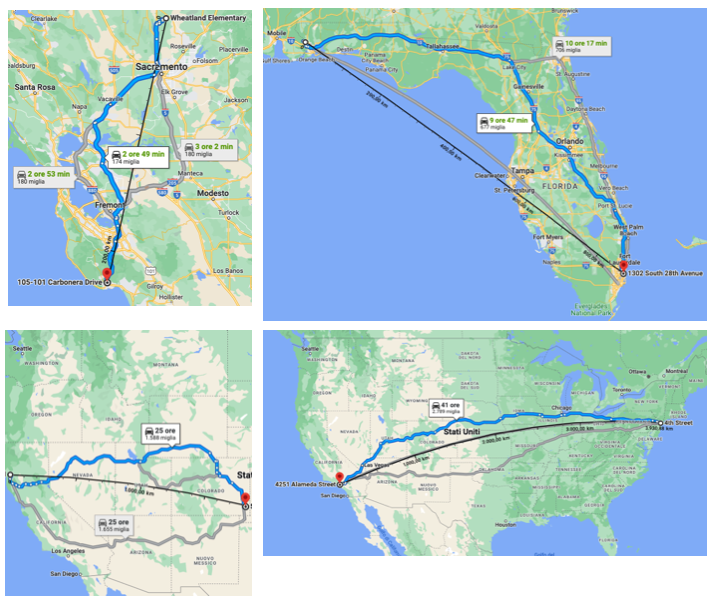
\includegraphics[width=0.75\linewidth]{google_maps.png}
			\caption{From left to right top to bottom BAY, FLA, W, USA}
			\label{testpaths}
		\end{figure}
	\end{frame}
	%% %%%%%%%%%%%%%%%%%%%%%%%% %%
	%% CHAPTER 4: SEQUENTIAL A* %%
	%% %%%%%%%%%%%%%%%%%%%%%%%% %%
	\begin{frame}
		\frametitle{4. Sequential A* Algorithm}
		%\framesubtitle{Pseudocode}
		The first step consists of a pre-computation of:
		\begin{itemize}
		\item The heurstic $h(n)$ for each node computed through the Haversine formula.
		\item The initial values of $f(n)$ and $g(n)$ that will be set to $DOUBLE\_MAX$ for each
				node except for the source node that will have $f(source) = h(source)$ and $g(source) = 0$.
		\end{itemize}
		Relevant data structures are:
		\begin{itemize}
			\item \textit{costToCome} table
			\item \textit{parentVertex} table
		  \end{itemize}
	\end{frame}

	\begin{frame}[allowframebreaks] 
		\frametitle{4. Sequential A* Algorithm}
		\begin{algorithmic}[1]
			\Function{$astar$}{$G, source, dest$}
			\State $g[i] \gets DOUBLE\_MAX \;\forall i \in V$\;
			\State $f[i] \gets DOUBLE\_MAX \;\forall i \in V$\;
			\State $h[i] \gets h(i, d) \; \forall i \in V$\;
			\State $parentVertex[i] \gets -1 \; \forall i \in V$\;
			\State $f[source] \gets h[ssource]$\;
			\State $g[source] \gets 0$\;
			\State $openSet := \{(source, f[source])\}$\;
			\While{$!openSet.EMPTY()$}
				\State $a \gets openSet.POP()$\;
			\If{$a == dest$}
				\State reconstructPath()\;
			\EndIf
			\ForAll{neighbors $b$ of $a$}
				\State $wt \gets weight(a, b)$\;
				\State $tentativeScore \gets g[a] + wt$\;
				\If{$tentativeScore < g[b]$}
					\State $parentVertex[b] \gets a$\;
					\State $costToCome[b] \gets wt$\;
					\State $g[b] \gets tentativeScore$\;
					\State $f[b] \gets g[b] + h[b]$\;
					\State $openSet.PUSH((b, f[b]))$\;
				\EndIf
			\EndFor
			\EndWhile
			\EndFunction
		  \end{algorithmic}
	\end{frame}

	\begin{frame}
		\frametitle{4. Sequential A* Algorithm}
		\framesubtitle{Results}
		\begin{table}[]
			%\caption{Sequential algorithms performance}
			\begin{tabular}{|l|l|l|l|l|l|}
			\hline
			\textbf{}    & \textbf{File Size} & \textbf{Reading} & \textbf{A*} & \textbf{Total} & \textbf{\begin{tabular}[c]{@{}l@{}}Reading \\ Impact\end{tabular}} \\ \hline
			\textbf{RND} & 2876B              & 0.0011s          & 0.0862s     & 1.1714s        & 1.2872\%                                                           \\ \hline
			\textbf{BAY} & 20.51MB            & 0.9365s          & 0.2349s     & 1.1714s        & 79.9477\%                                                          \\ \hline
			\textbf{FLA} & 69.09MB            & 3.0728s          & 0.5893s     & 3.6621s        & 83.9075\%                                                          \\ \hline
			\end{tabular}
		\end{table}
		TODO why we need parallel reading...
	\end{frame}
	%% %%%%%%%%%%%%%%%%%%%%%%%%% %%
	%% CHAPTER 5: A* vs DIJKSTRA %%
	%% %%%%%%%%%%%%%%%%%%%%%%%%% %%
	\begin{frame}
		\frametitle{5. A* and Dijkstra: a comparison}
		\framesubtitle{Results}
		\begin{table}[ht!]
			%\caption{Expanded nodes vs total nodes for Dijkstra and A*}
			\begin{tabular}{|l|l|l|}
			\hline
			\textbf{Expanded nodes} & \textbf{Dijkstra} & \textbf{Sequential A*}       \\ \hline
			\textbf{RND}            & 15 of 101         & 13 of 101         \\ \hline
			\textbf{BAY}            & 318725 of 321270  & 156950 of 321270  \\ \hline
			\textbf{FLA}            & 996956 of 1070376 & 591926 of 1070376 \\ \hline
			\end{tabular}
		\end{table}
		TODO We can notice that...
	\end{frame}
	\begin{frame}
		\frametitle{5. A* and Dijkstra: a comparison}
		\framesubtitle{Results}
		\begin{figure}[ht!]
			\centering
			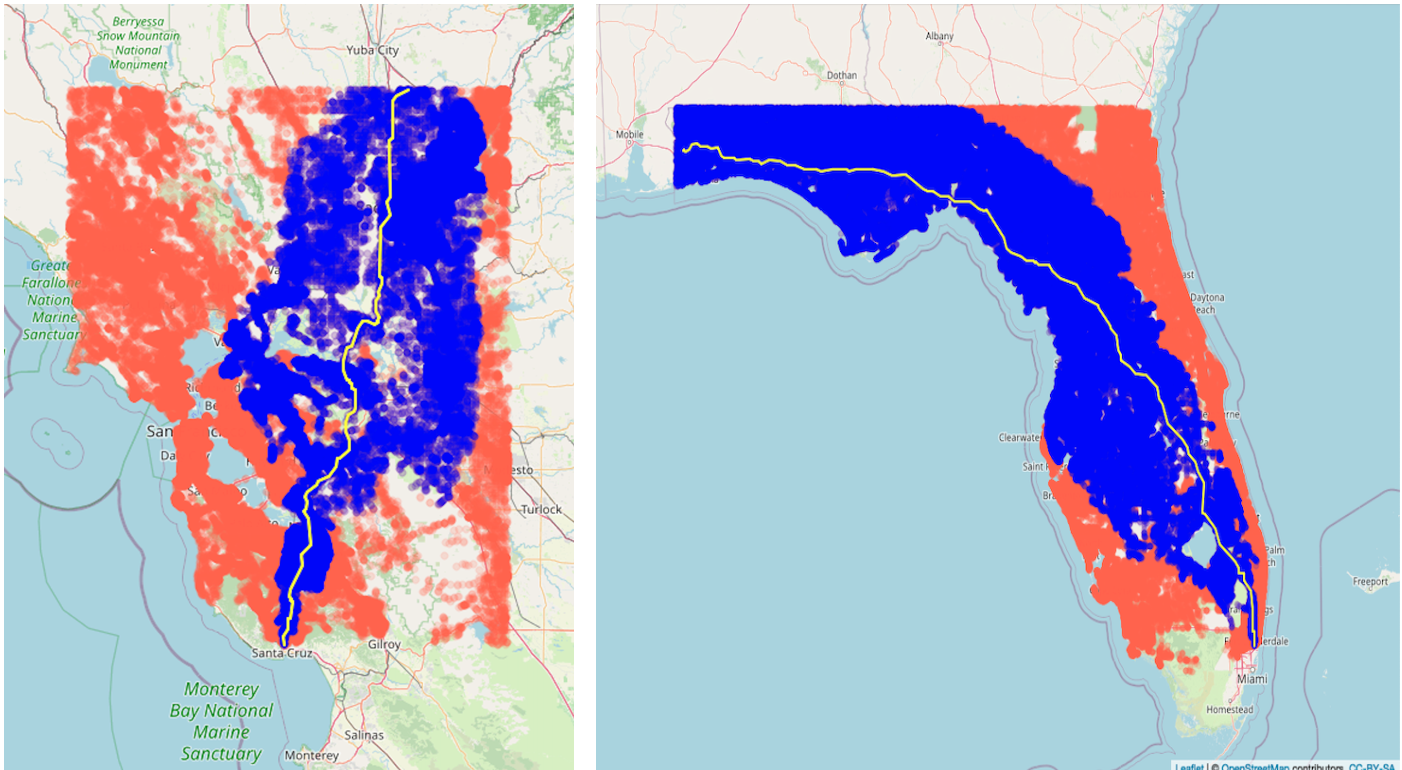
\includegraphics[width=1\linewidth]{dijkstra_astar.png}
			\caption{Test paths on BAY(left) and FLA(right)}
			\label{astardijkstra}
		\end{figure}
	\end{frame}
	%% %%%%%%%%%%%%%%%%%%%%%%%% %%
	%% CHAPTER 6: PARALLEL READ %%
	%% %%%%%%%%%%%%%%%%%%%%%%%% %%
	\begin{frame}
		\frametitle{6. Parallel reading of the input file}
		\framesubtitle{Parallel Read: approach 1}
		In this first approach we have implemeted a solution on which:
		\begin{itemize}
		\item $N$ threads runs freely to read the entire file
		\item Only one file descriptor is shared among all the threads (this means that
				when thread $t_i$ performs a \texttt{read} opearation all the other threads 
				are waiting for it to finish)
		\end{itemize}
	\end{frame}
	\begin{frame}
		\frametitle{6. Parallel reading of the input file}
		\framesubtitle{Parallel Read: approach 1 - Results on FLA map}
		\begin{figure}[ht!]
			\centering
			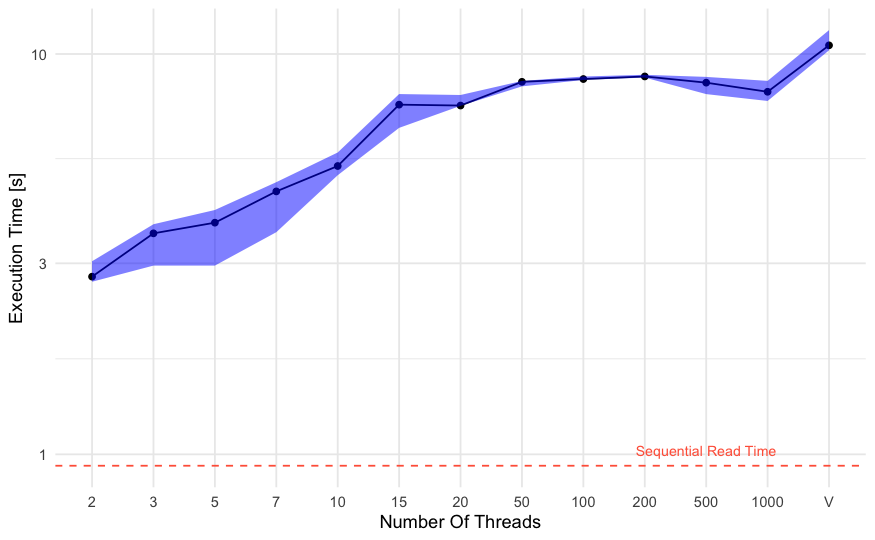
\includegraphics[width=1\linewidth]{par_read_1_time.png}
			%\caption{Performance of approach 1 for different number of threads}
			\label{parread1time}
	 	 \end{figure}	
	\end{frame}
	\begin{frame}
		\frametitle{6. Parallel reading of the input file}
		\framesubtitle{Parallel Read: approach 2}
		TODO explain...
	\end{frame}
	\begin{frame}
		\frametitle{6. Parallel reading of the input file}
		\framesubtitle{Parallel Read: approach 2 - Results on FLA map}
		\begin{figure}[ht!]
			\centering
			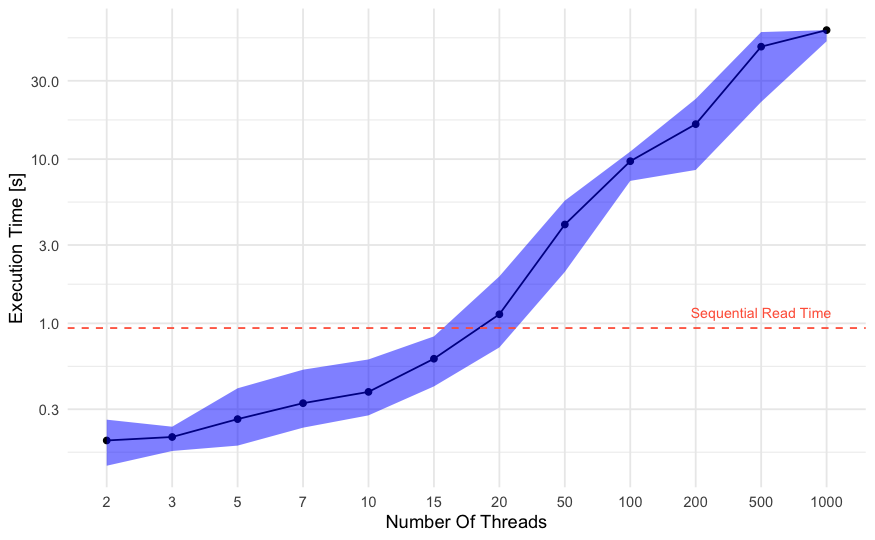
\includegraphics[width=1\linewidth]{par_read_2_time.png}
			%\caption{Performance of approach 2 for different number of threads}
			\label{parread2time}
		  \end{figure}
	\end{frame}
	\begin{frame}
		\frametitle{6. Parallel reading of the input file}
		\framesubtitle{Parallel Read: approach 3}
		\begin{itemize}
			\item Letting threads differentiate among \textit{nodes section} and 
				  \textit{edges section} to be able to read them togheter.
			\item Using a $(NP, NT)$ mechanism to read each section of the input file (where
				  $NP$ is the number of partitions the section is divided in and $NT$ is the number
				  of threads that have to read all the partitions).
		\end{itemize}
	\end{frame}
	\begin{frame}
		\frametitle{6. Parallel reading of the input file}
		\framesubtitle{Parallel Read: approach 3}
		\begin{figure}[ht!]
			\centering
			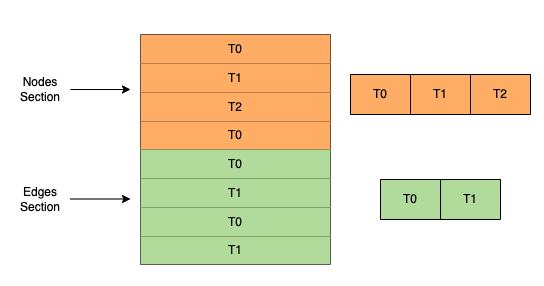
\includegraphics[width=0.75\linewidth]{par_read_3.png}
			%\caption{Example of parallel read - approach 3}
			\label{parread3}
		  \end{figure}
	\end{frame}
	\begin{frame}
		\frametitle{6. Parallel reading of the input file}
		\framesubtitle{Parallel Read: approach 3 - Results on FLA map}
		\begin{figure}[ht!]
			\centering
			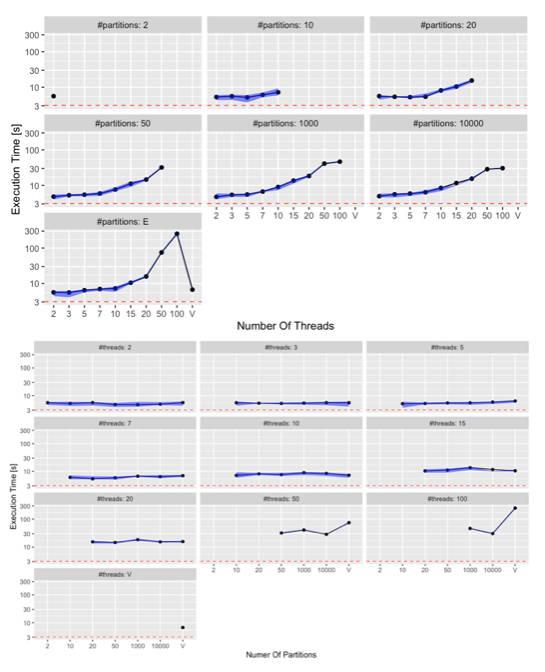
\includegraphics[width=0.5\linewidth]{par_read_3_time.png}
			%\caption{Performance of approach 3 for different number of threads and partitions}
			\label{parread3time}
		\end{figure}
	\end{frame}
	\begin{frame}
		\frametitle{6. Parallel reading of the input file}
		\framesubtitle{Final Results on FLA map}
		\begin{figure}[ht!]
			\centering
			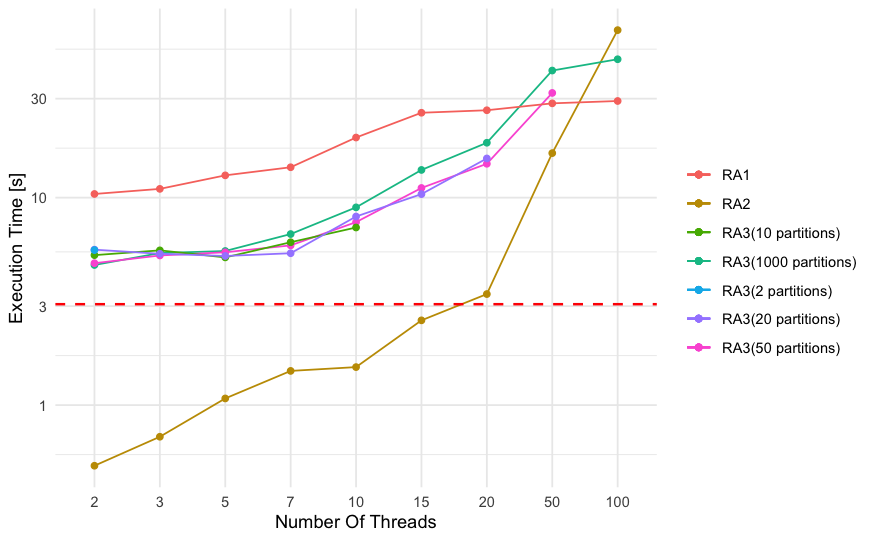
\includegraphics[width=1\linewidth]{par_read_all_time.png}
			\caption{RA(Read Approach) 1,2,3 compared with sequential reading}
			\label{parreadalltime}
		\end{figure}
	\end{frame}
	\begin{frame}
		\frametitle{6. Parallel reading of the input file}
		\framesubtitle{Best performing model results}
		By using the most effective model we have found, Parallel Read Approach 2 with 2 threads,
		we have measured time performance over all the benchmark files:
		\begin{table}[ht!]
			\centering
			  %\caption{RA2 results against sequential reading}
			  \begin{tabular}{|l|l|l|l|}
			  \hline
			  \textbf{}    & \textbf{\begin{tabular}[c]{@{}l@{}}RA2\\ (2 threads)\end{tabular}} & \textbf{Sequential} & \textbf{Speed-Up} \\ \hline
			  \textbf{BAY} & 0.1936s                                                            & 0.9366s             & 79.3\%            \\ \hline
			  \textbf{FLA} & 0.5103s                                                            & 3.0650s             & 83.4\%            \\ \hline
			  \textbf{USA} & 14.1492s                                                           & 56.4445s            & 74.9\%            \\ \hline
			  \end{tabular}
			  \label{readresultsfinal}
		  \end{table}
	\end{frame}
	%% %%%%%%%%%%%%%%%%%%%%%% %%
	%% CHAPTER 7: PARALLEL A* %%
	%% %%%%%%%%%%%%%%%%%%%%%% %%
	\begin{frame}
		\frametitle{7. Parallel A*}
		The goal of the project was to find one or more parallel versions of the A* algorithm 
		and showing their performances w.r.t. the sequential version. We have choosen three approaches
		to face the problem of parallelizing the A* algorithm: 
		\begin{itemize}
			\item \textbf{First Attempt (FA)}: a trivial algorithm that simply
				  works as the sequential algorithm but gives the possibility of executing it in a multithread
			      fashion by sharing the common data structure \textit{OPEN SET} among a variable number
				  of threads.
			\item \textbf{Hash Distributed A* (HDA*)}: it puts in action a more
				  complex way of parallelizing A* by defining a hash-based work distribution strategy.
		    \item \textbf{Parallel New Bidirectional A* (PNBA*)}: parallel search of the path from \textit{source} to \textit{dest}
				  and of the path from \textit{dest} to \textit{source} in the reversed graph.
		\end{itemize}
	\end{frame}
	\begin{frame}
		\frametitle{7. Parallel A*}
		\framesubtitle{First Attempt (FA)}

	\end{frame}
	\begin{frame}
		\frametitle{7. Parallel A*}
		\framesubtitle{HDA}

	\end{frame}
	\begin{frame}
		\frametitle{7. Parallel A*}
		\framesubtitle{PNBA*}

	\end{frame}


\end{document}